\newpage
\section{HISTORY}

\thispagestyle{main}
\subsection{Introduction to the History}

This is a history of my topic. See Figure \ref{Fig2} for an example of using the tikz package to draw figures on the fly.

\lipsum[6]               % generates dummy text


%%%%%%%%%%%%%%%%%
%  Tikz image
%%%%%%%%%%%%%%%%%

\begin{figure}[htb]
\centering
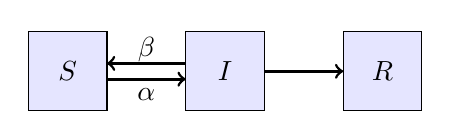
\begin{tikzpicture}[scale=1]
% Draw box
\draw[fill=blue!10]  (0,0)--(1,0) -- (1,1)--(0,1)--cycle;
% Put letter in middle of box
\draw (0.5,0.5) node {$S$};

% More boxes
\draw[fill=blue!10]  (2,0)--(3,0) -- (3,1)--(2,1)--cycle;
\draw (2.5,0.5) node {$I$};

\draw[fill=blue!10]  (4,0)--(5,0) -- (5,1)--(4,1)--cycle;
\draw (4.5,0.5) node {$R$};

% Add arrows

\draw[->,line width = 1] (1,0.4)--(2,0.4);
\draw[<-,line width = 1] (1,0.6)--(2,0.6);

\draw[->,line width = 1] (3,0.5)--(4,0.5);

\draw (1.5,0.5) node[above] {$\beta$};
\draw (1.5,-0) node[above] {$\alpha$};
\end{tikzpicture}
\caption{Example of using tikz package.}\label{Fig2}
\end{figure}

\lipsum[7]               % generates dummy text

%%%%%%%%%%%%%%%%%
%  Table
%%%%%%%%%%%%%%%%%

\begin{table}[htb]
\begin{center}
\begin{tabular}{ l | c | r }
  \hline			
  1 & 2 & 3 \\
  4 & 5 & 6 \\
  7 & 8 & 9 \\
  \hline  
\end{tabular}
\caption{Example of a table.}
\label{Tab1}
\end{center}
\end{table}

\lipsum[8]               % generates dummy text


